\section{分布表示的边界}
\label{sec:rvd-representation-limits}

到目前为止，每个例子要么能列成一张概率表，要么有密度。是不是所有随机变量都属于这两类之一？先看一个很平常的等待问题，它两类都不属于。

\paragraph{有时不用等}
顾客来到窗口时，若窗口恰好空闲（概率$0.3$），等待时间为$0$；否则等待时间按式~\eqref{eq:rvd-waiting-cdf}的规律分布。记等待时间为$W$。由全概率公式，对$t\geq0$，
\[
  \mathbb{P}(W\leq t)=0.3\cdot1+0.7\,(1-\mathrm{e}^{-t}),
\]
其中第一项是窗口空闲、等待为$0$的情形，第二项是窗口忙、等待不超过$t$的情形。于是
\begin{equation}
  F_W(t)=\begin{cases}0,&t<0,\\0.3+0.7\,(1-\mathrm{e}^{-t}),&t\geq0.\end{cases}
  \label{eq:rvd-mixed-cdf}
\end{equation}
图~\ref{fig:rvd-mixed-cdfs}(a)画出了这条曲线：它在$0$处从$0$跳到$0.3$，之后连续上升。

\begin{BookInlineFigure}
  \centering
  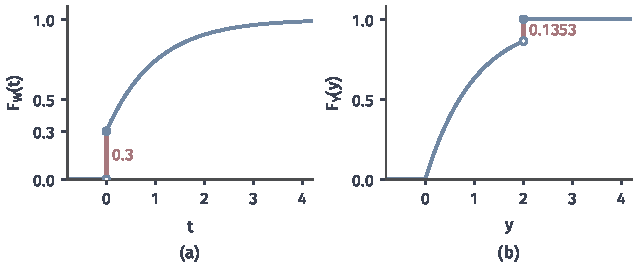
\includegraphics[width=108mm]{figures/07-probability/01-elementary-probability/matplotlib/rvd-mixed-cdfs/figure.pdf}
  \caption{既有跳跃又有连续上升的分布函数。(a)可能不用等的等待时间$W$，在$0$处跳跃$0.3$（红线），之后按$0.7(1-\mathrm{e}^{-t})$连续增加；(b)截断的等待时间$Y=\min\{T,2\}$，在$[0,2)$上与$1-\mathrm{e}^{-y}$相同，在$2$处跳跃$\mathrm{e}^{-2}\approx0.1353$。空心点是左极限，实心点是函数值。}
  \label{fig:rvd-mixed-cdfs}
\end{BookInlineFigure}

$W$不是离散随机变量。按模型，$0$这一点带有概率$0.3$；分布函数在其余各点连续，用第~\ref{sec:rvd-mass-density}节对等待时间所用的夹逼，其余每一点的概率都是$0$；可数个点上的质量加起来至多$0.3$，凑不满$1$。$W$也没有密度。若有密度，定理~\ref{thm:rvd-density-cdf}要求$\mathbb{P}(W=0)=0$，与$0.3$矛盾。概率表和密度都只能描述$W$的一部分质量。

计算时把两部分分开处理：跳跃部分求和，连续部分积分。对区间$B$，
\begin{equation}
  \mathbb{P}(W\in B)=0.3\cdot\mathbf{1}_{B}(0)+0.7\int_{B\cap(0,\infty)}\mathrm{e}^{-t}\,\mathrm{d}t,
  \label{eq:rvd-mixed-prob}
\end{equation}
其中$\mathbf{1}_{B}(0)$在$0\in B$时为$1$，否则为$0$。下面用三个区间演示。是否包含$0$决定了第一项：
\[
  \mathbb{P}(W\leq1)=0.3+0.7(1-\mathrm{e}^{-1})\approx0.7425,
\]
\[
  \mathbb{P}(0<W\leq1)=0.7(1-\mathrm{e}^{-1})\approx0.4425 .
\]
远离$0$的区间只有第二项，例如$\mathbb{P}(W>2)=0.7\,\mathrm{e}^{-2}\approx0.0947$。

分位数照样按式~\eqref{eq:rvd-quantile}计算。$p\leq0.3$时，$F_W(0)=0.3\geq p$而$t<0$时$F_W(t)=0$，所以$Q(p)=0$：有三成顾客根本不用等。$p>0.3$时解$0.3+0.7(1-\mathrm{e}^{-t})=p$，得
\[
  Q(p)=\ln\frac{0.7}{1-p},\qquad 0.3<p<1 .
\]
中位数是$\ln(7/5)\approx0.336$分钟，比不考虑空闲时的$\ln2\approx0.693$分钟短。

\paragraph{截断产生的跳跃}
这类分布并不罕见，对有密度的变量取函数就可能产生。设顾客最多等$2$分钟，等不到就离开，记录到的时长是$Y=\min\{T,2\}$。$y<2$时$\{Y\leq y\}=\{T\leq y\}$；$y\geq2$时$Y\leq y$总成立。所以
\[
  F_Y(y)=\begin{cases}0,&y<0,\\1-\mathrm{e}^{-y},&0\leq y<2,\\1,&y\geq2.\end{cases}
\]
它在$2$处跳跃，跳跃高度$\mathrm{e}^{-2}\approx0.1353$就是$\mathbb{P}(T\geq2)$：所有等待超过$2$分钟的质量都被堆到了$2$这一点上（图~\ref{fig:rvd-mixed-cdfs}(b)）。测量仪器有量程上限、记录有截止时间时，都会出现这种情形。

$Y$的分位数显示出跳跃的另一面。$p\leq1-\mathrm{e}^{-2}\approx0.8647$时，方程$1-\mathrm{e}^{-y}=p$在$[0,2)$中有解，$Q_Y(p)=-\ln(1-p)$，与$T$的分位数相同；$p>0.8647$时，累计概率在$y=2$处才首次达到$p$，$Q_Y(p)=2$。分布函数在$2$处的跳跃，变成了分位数函数在$(0.8647,1)$上的平台。截断只改变了高分位数，中位数仍是$\ln2$。

\paragraph{分离跳跃}
两个例子都由“跳跃部分”和“连续部分”组成。这种分离对任何分布函数都可以做到：先证明跳跃只能有可数个，再把它们集中成一张概率表，剩下的部分连续。

\begin{theorem}[分布函数的跳跃分解]
\label{thm:rvd-jump-decomposition}
设$F$单调不减、右连续，且$\lim_{x\to-\infty}F(x)=0$，$\lim_{x\to+\infty}F(x)=1$。记$J(a)=F(a)-F(a^{-})$为$a$处的跳跃高度。则
\begin{enumerate}
  \item 跳跃点$\{a:J(a)>0\}$至多可数，且跳跃高度的总和不超过$1$；
  \item 令
  \begin{equation}
    F_{\mathrm{d}}(x)=\sum_{a\leq x}J(a),\qquad F_{\mathrm{c}}(x)=F(x)-F_{\mathrm{d}}(x),
    \label{eq:rvd-jump-parts}
  \end{equation}
  则$F_{\mathrm{c}}$单调不减且处处连续。
\end{enumerate}
\end{theorem}

\begin{proof}
先看有限个跳跃点$a_1<a_2<\dots<a_m$。对相邻的两点，单调性给出$F(a_k)\leq F(a_{k+1}^{-})$，所以各段增量
\[
  F(a_m)-F(a_1^{-})=\sum_{k=1}^{m}J(a_k)+\sum_{k=1}^{m-1}\bigl(F(a_{k+1}^{-})-F(a_k)\bigr)\geq\sum_{k=1}^{m}J(a_k).
\]
左边不超过$1$，所以任意有限个跳跃高度之和不超过$1$。

固定正整数$n$。若有$m$个点的跳跃高度都大于$1/n$，则$m/n<1$，即$m<n$。所以跳跃高度大于$1/n$的点少于$n$个。全部跳跃点是这些有限集对$n=1,2,\dots$的并，因而至多可数；任意有限部分和不超过$1$，总和也不超过$1$。

再看$F_{\mathrm{c}}$。对$x<y$，把上面的论证用在$(x,y]$中有限个跳跃点上，再取上确界，得到
\[
  F(y)-F(x)\geq\sum_{x<a\leq y}J(a)=F_{\mathrm{d}}(y)-F_{\mathrm{d}}(x),
\]
即$F_{\mathrm{c}}(y)\geq F_{\mathrm{c}}(x)$。

$F_{\mathrm{d}}$与离散变量的分布函数结构相同：可数个点$a$各带非负质量$J(a)$，只是总量可能小于$1$。定理~\ref{thm:rvd-cdf-properties}中右连续与左极限的证明只用到质量非负、总和有限，所以$F_{\mathrm{d}}$右连续，并且在$a$处的跳跃恰为$J(a)$。$F$本身右连续、在$a$处跳跃$J(a)$，二者相减，$F_{\mathrm{c}}$右连续且在每点的跳跃为$0$，即处处连续。
\end{proof}

对$W$，$F_{\mathrm{d}}(t)=0.3\cdot\mathbf{1}_{\{t\geq0\}}$，连续部分在$t\geq0$时为$0.7(1-\mathrm{e}^{-t})$，它有密度$0.7\,\mathrm{e}^{-t}$，式~\eqref{eq:rvd-mixed-prob}正是按这一分解写成的。对$Y$，跳跃部分是$2$处的$\mathrm{e}^{-2}$，连续部分在$[0,2]$上由密度$\mathrm{e}^{-y}$积分得到。那么，连续部分是不是总有密度？

\paragraph{分布函数连续也未必有密度}
下面构造一个分布函数处处连续、却没有密度的随机变量。反复抛一枚公平硬币，各次独立，第$k$次正面记$D_k=1$，反面记$D_k=0$。令
\begin{equation}
  X=\sum_{k=1}^{\infty}\frac{2D_k}{3^{k}} .
  \label{eq:rvd-cantor}
\end{equation}
级数各项不超过$2/3^{k}$，总是收敛，$X\in[0,1]$。用三进制看，$X$的第$k$位小数是$2D_k$，只取$0$或$2$，永远不取$1$。

前$n$次抛掷决定了$X$落在哪一段。前$n$项的和是若干个$2/3^{k}$之和，剩余各项之和满足
\[
  0\leq\sum_{k>n}\frac{2D_k}{3^{k}}\leq\sum_{k>n}\frac{2}{3^{k}}=\frac{1}{3^{n}},
\]
所以$X$落在以前$n$项之和为左端点、长$3^{-n}$的闭区间里。前$n$次抛掷有$2^{n}$种等可能的结果，对应$2^{n}$个这样的区间，每个的概率是$2^{-n}$。

这些区间可以一层层画出来（图~\ref{fig:rvd-cantor-split}）。第一层是$[0,1/3]$和$[2/3,1]$，由$D_1=0$或$1$决定，各得一半质量；中间的$(1/3,2/3)$对应三进制首位为$1$，得不到任何质量。下一层把每个保留的区间再三等分，质量对半分给左右两段，中间一段又是空的。记第$n$层的$2^{n}$个区间之并为$C_n$，则$\mathbb{P}(X\in C_n)=1$，而$C_n$的总长度是$(2/3)^{n}$。

\begin{BookInlineFigure}
  \centering
  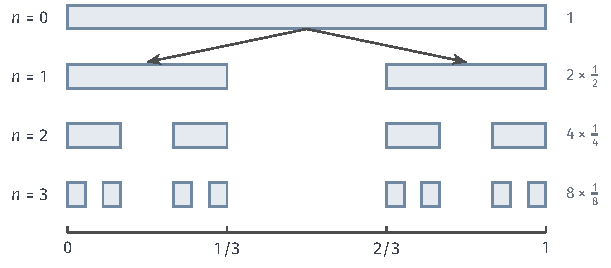
\includegraphics[width=104mm]{figures/07-probability/01-elementary-probability/tikz/rvd-cantor-split/figure.pdf}
  \caption{式~\eqref{eq:rvd-cantor}中$X$的质量怎样一层层分配。第$n$层有$2^{n}$个长$3^{-n}$的区间，每个区间的质量平分给它的左右两个三分之一，中间三分之一得不到质量。右侧是每层区间的个数与各自的质量；第$n$层总长$(2/3)^{n}$，总质量始终为$1$。}
  \label{fig:rvd-cantor-split}
\end{BookInlineFigure}

第一个结论：$F_X$处处连续。同一层的区间彼此之间至少隔着长$3^{-n}$的空档，所以长度小于$3^{-n}$的任何区间至多与该层的两个区间相交。对任意$x$和$0<h<3^{-n}/2$，区间$(x-h,x+h]$长度小于$3^{-n}$，于是
\[
  F_X(x+h)-F_X(x-h)=\mathbb{P}(x-h<X\leq x+h)\leq2\cdot2^{-n}.
\]
$n$可以任意大，所以$h\to0$时这个差趋于$0$，$F_X$在$x$处连续。特别地，每个单点的概率都是$0$，$X$不是离散随机变量。

第二个结论：$X$没有有界的密度。若$X$有密度$f$且$f\leq K$，则$X$落在$C_n$的概率是$f$在这$2^{n}$个区间上的积分之和，不超过$K$乘总长度：
\[
  1=\mathbb{P}(X\in C_n)\leq K\Bigl(\frac23\Bigr)^{n}.
\]
令$n\to\infty$，右边趋于$0$，矛盾。直观地说，全部质量挤在总长度任意小的集合上，单位长度上的概率只能无限大。

去掉“有界”这个限制，结论仍然成立：$X$根本没有密度。对无界的被积函数，上面的估计不再可用，严格证明需要比黎曼积分更一般的积分理论，可参考\BookChapterRef{chap:measure-densities}{卷四第8章“测度的密度”}。从分布函数一侧也能看到问题所在：$F_X$在被删去的每个中间三分之一上都是常数（那里没有质量），这些开区间的总长度是$1-(2/3)^{n}\to1$，所以$F_X$的导数在总长为$1$的范围内都是$0$；然而$F_X$从$0$升到了$1$。对导数积分只会得到$0$。定理~\ref{thm:rvd-cdf-to-density}的途径在这里失效，因为它要求除有限个点外可导。而对每一层都被保留的点$x$，包含$x$的第$n$层区间长$3^{-n}$，$F_X$在其上增加$2^{-n}$，差商为$(3/2)^{n}$，随$n$增大趋于无穷，所以$F_X$在这些点处不可导，这样的点有无穷多个。

图~\ref{fig:rvd-cantor-cdf}画出了$F_X$，它称为Cantor函数，$X$的分布称为\term{Cantor分布}（Cantor distribution）。黄线和紫线是把第$1$、$2$层的质量在各区间内均匀铺开得到的分布函数，蓝线是极限。每加细一层，上升的部分被压缩到更短的区间里，坡度变陡，平台变多。

\begin{BookInlineFigure}
  \centering
  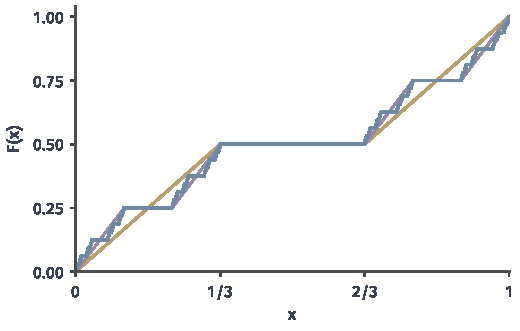
\includegraphics[width=88mm]{figures/07-probability/01-elementary-probability/matplotlib/rvd-cantor-cdf/figure.pdf}
  \caption{Cantor分布的分布函数（蓝线）。黄线与紫线分别把第$1$层、第$2$层区间上的质量均匀铺开，坡度为$(3/2)^{n}$。极限曲线连续，从$0$升到$1$，却在总长为$1$的一组区间上保持水平。}
  \label{fig:rvd-cantor-cdf}
\end{BookInlineFigure}

这个例子是专门构造出来的，在建模中很少直接出现。它说明的是一条边界：离散分布、有密度的分布以及二者的组合，并没有穷尽全部分布。一般的分布函数在去掉跳跃部分之后，连续部分还可以再分成有密度的部分和像Cantor函数这样没有密度的部分，相应的分解定理在卷四的同一章中给出。

\paragraph{各种表示的适用范围}
图~\ref{fig:rvd-representations}把本章的例子放到一起。分布函数对所有分布都存在；概率表只适用于离散分布；密度只适用于有密度的分布；像$W$和$Y$那样的分布需要两者组合；Cantor分布的分布函数连续，却两者都用不上。

\begin{BookInlineFigure}
  \centering
  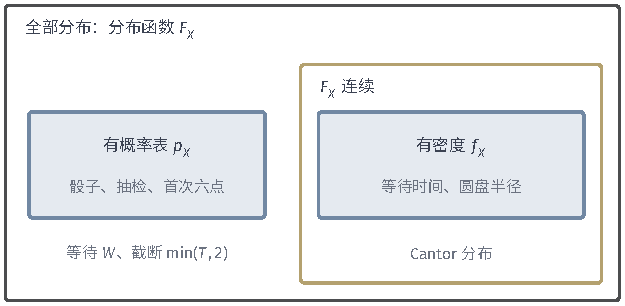
\includegraphics[width=105mm]{figures/07-probability/01-elementary-probability/tikz/rvd-representations/figure.pdf}
  \caption{各种表示的适用范围。外框是全部分布，它们都有分布函数；左侧蓝框是有概率表的离散分布，右侧黄框是分布函数连续的分布，其中蓝框是有密度的分布。框外标注的是两者都不适用的例子：可能不用等的$W$与截断的$\min\{T,2\}$既有跳跃又有连续部分，Cantor分布连续却没有密度。}
  \label{fig:rvd-representations}
\end{BookInlineFigure}

要对所有这些情形使用同一种语言，就不能再依赖“求和”与“黎曼积分”这两种具体的计算方式，而要直接把分布看作对实轴子集赋予概率的规则，并为它建立统一的积分。第~\ref{chap:probability-spaces}章完成这件事：概率表、密度以及它们的组合都成为同一种对象的特例，Cantor分布也能放进同一框架。在那之前，本部分只使用离散模型、密度模型以及按式~\eqref{eq:rvd-mixed-prob}那样分开计算的组合。
